\documentclass{article}
\usepackage{hyperref}
\usepackage{subfiles}
\usepackage{amsmath}
\usepackage{graphicx}
\usepackage{caption}
\usepackage{subcaption}
\usepackage{multirow}
\usepackage{booktabs}
\usepackage{rotating}
\usepackage{pgfplotstable}
\usepackage{siunitx} % Required for alignment
\sisetup{
  round-mode          = places, % Rounds numbers
  round-precision     = 2, % to 2 places
}
\subfile{cover.tex}

\begin{document}
\pagenumbering{gobble}
\maketitle
\newpage
\tableofcontents
\pagenumbering{roman}
\newpage
\listoffigures
\listoftables
\newpage
\pagenumbering{arabic}

\section{Very Important Section}
Hello world \LaTeX
\url{https://linuxconfig.org}

\subsection{Things Bulleted}
\begin{itemize}
	\item Thing 1
	\item Thing 2
\end{itemize}

\subsection{Things Enumerated}
\begin{enumerate}
	\item Thing 1
	\item Thing 2
\end{enumerate}

\subsection{Equations}
\begin{align*}
  f(x) &= x^2\\
  g(x) &= \frac{1}{x}\\
  F(x) &= \int^a_b \frac{1}{3}x^3
\end{align*}

\subsection{Matrices}
\begin{align*}
\begin{bmatrix}
	1 & 2 & 3\\
	a & b & c
\end{bmatrix}
\end{align*}

\section{Oh Pretty Pictures}
Look at the pretty pictures

\subsection{Pretty Pictures}
\begin{figure}[b!]
	\centering
	\begin{subfigure}[b]{0.3\linewidth}
		\centering
		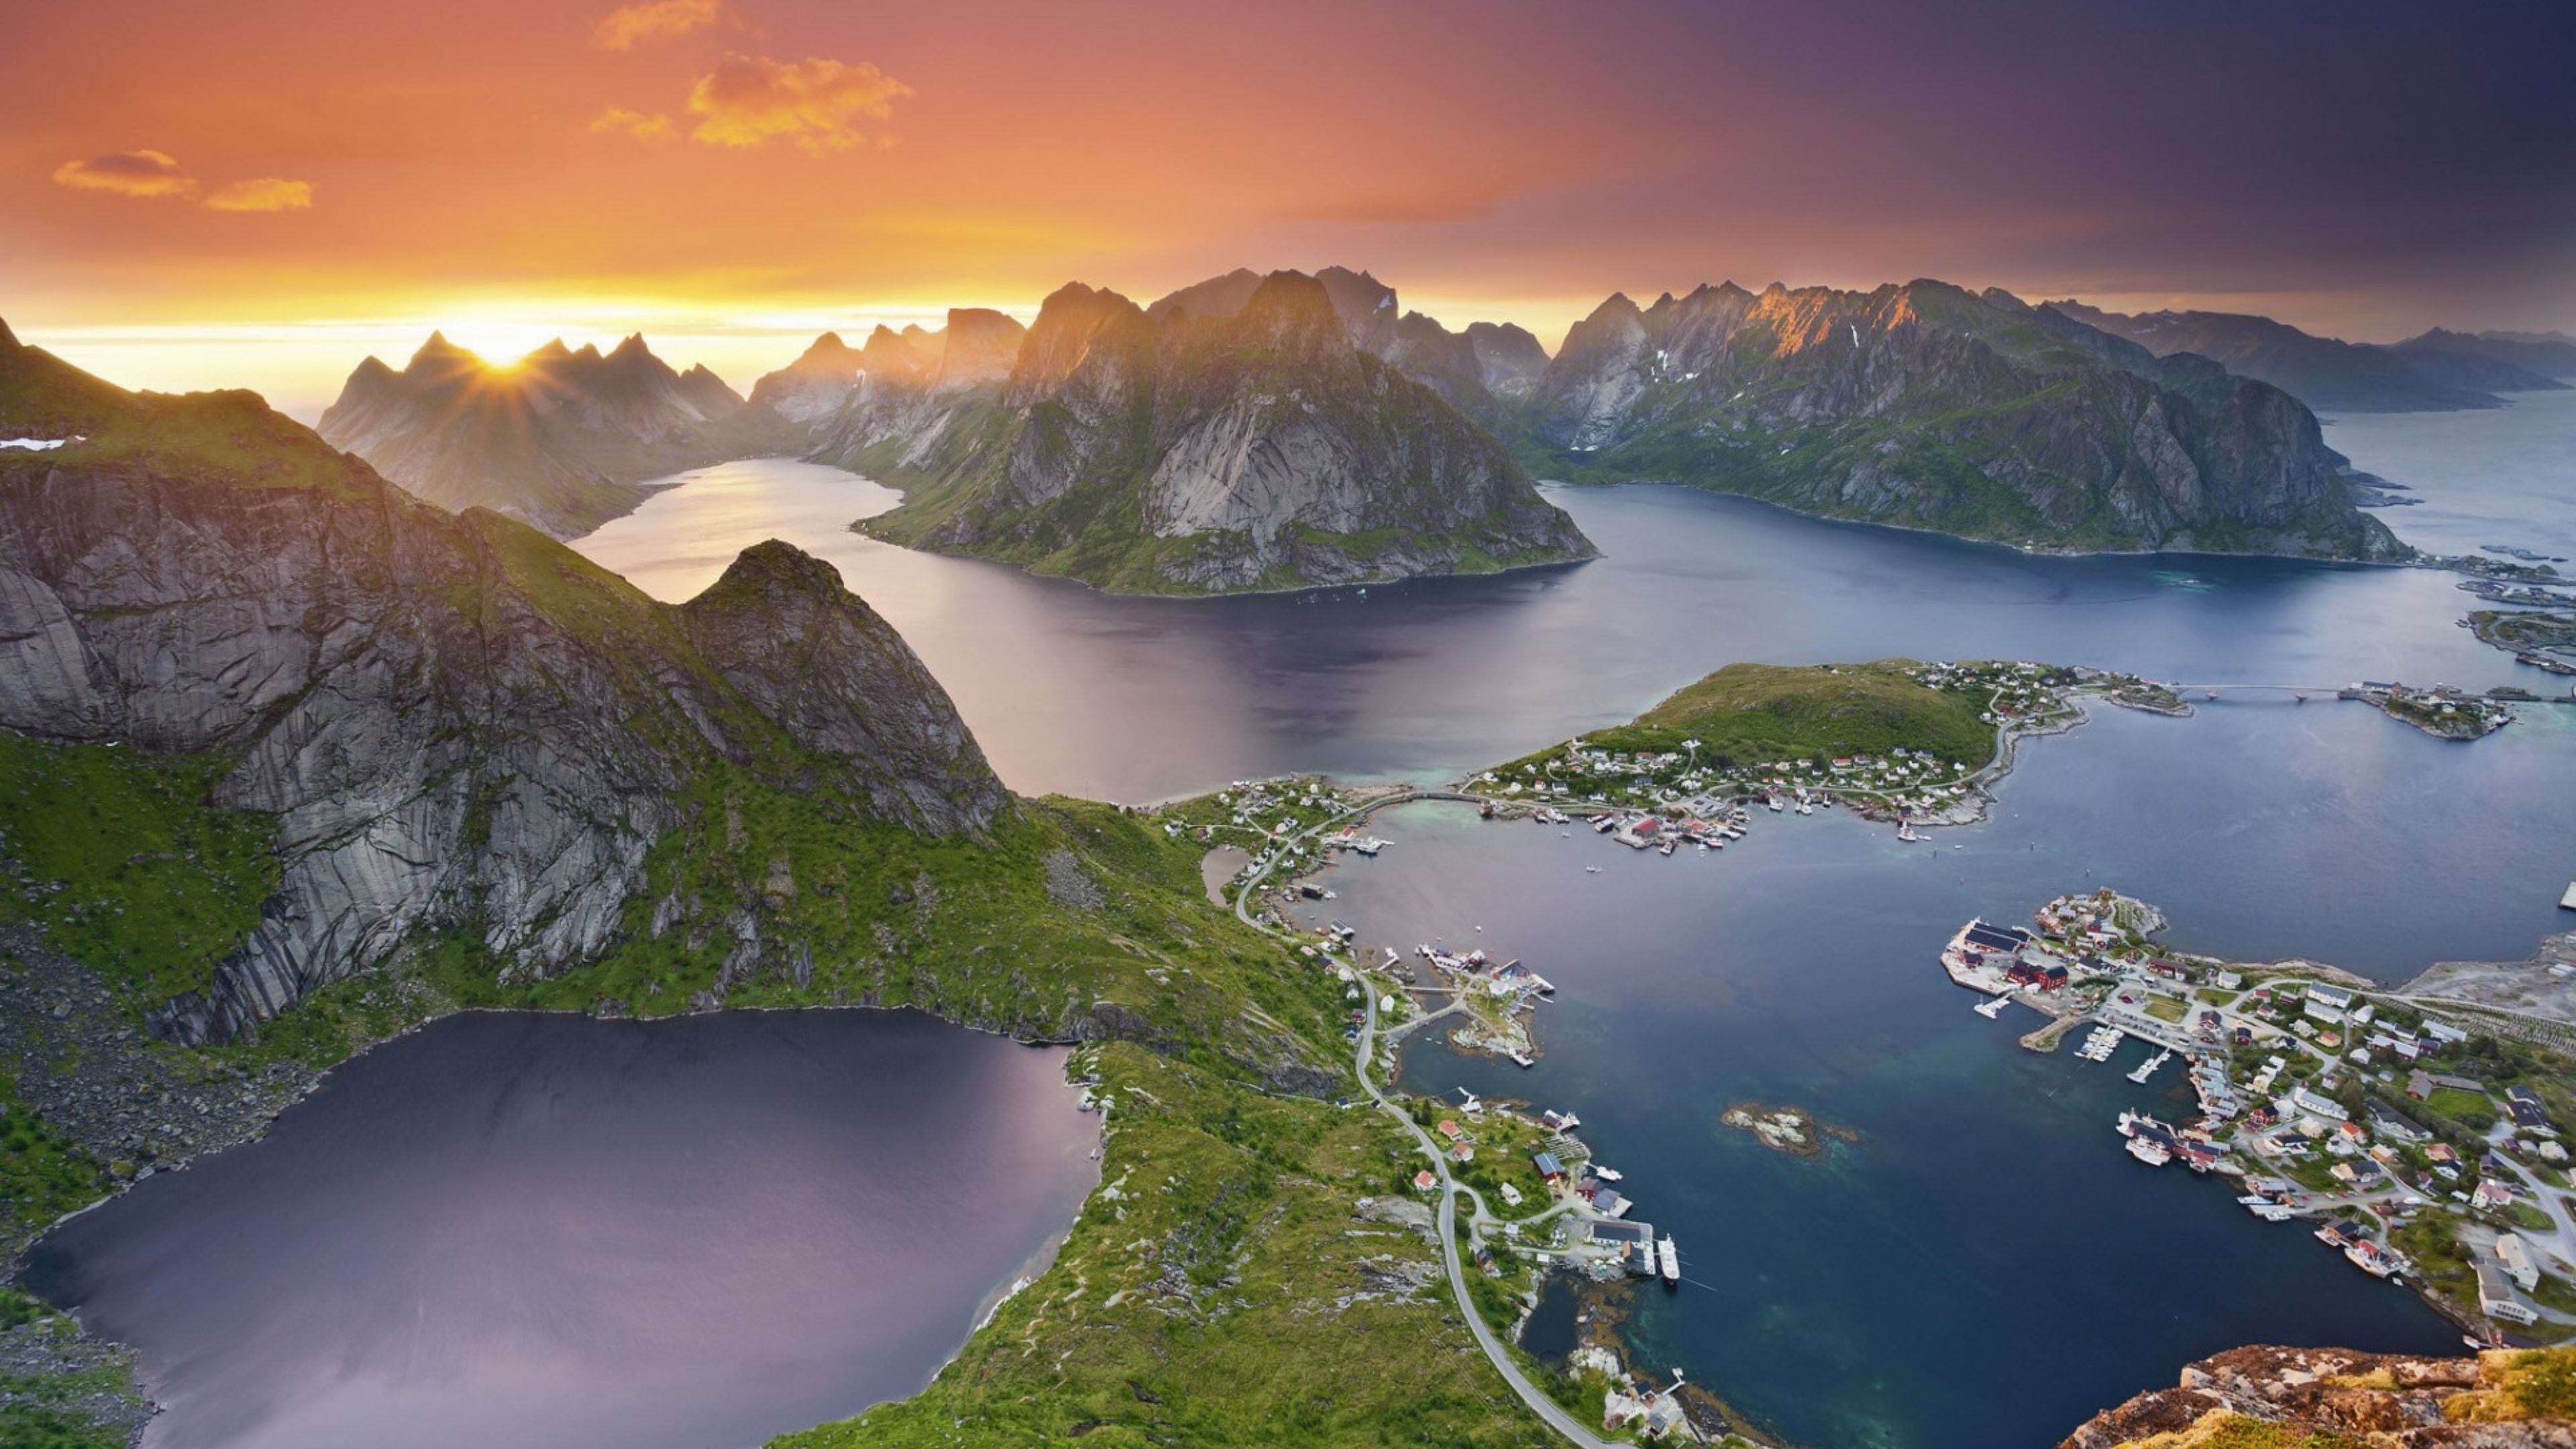
\includegraphics[width=\linewidth]{imgs/Norge1.jpg}
		\caption{Norge}
	\end{subfigure}
	\begin{subfigure}[b]{0.3\linewidth}
		\centering
		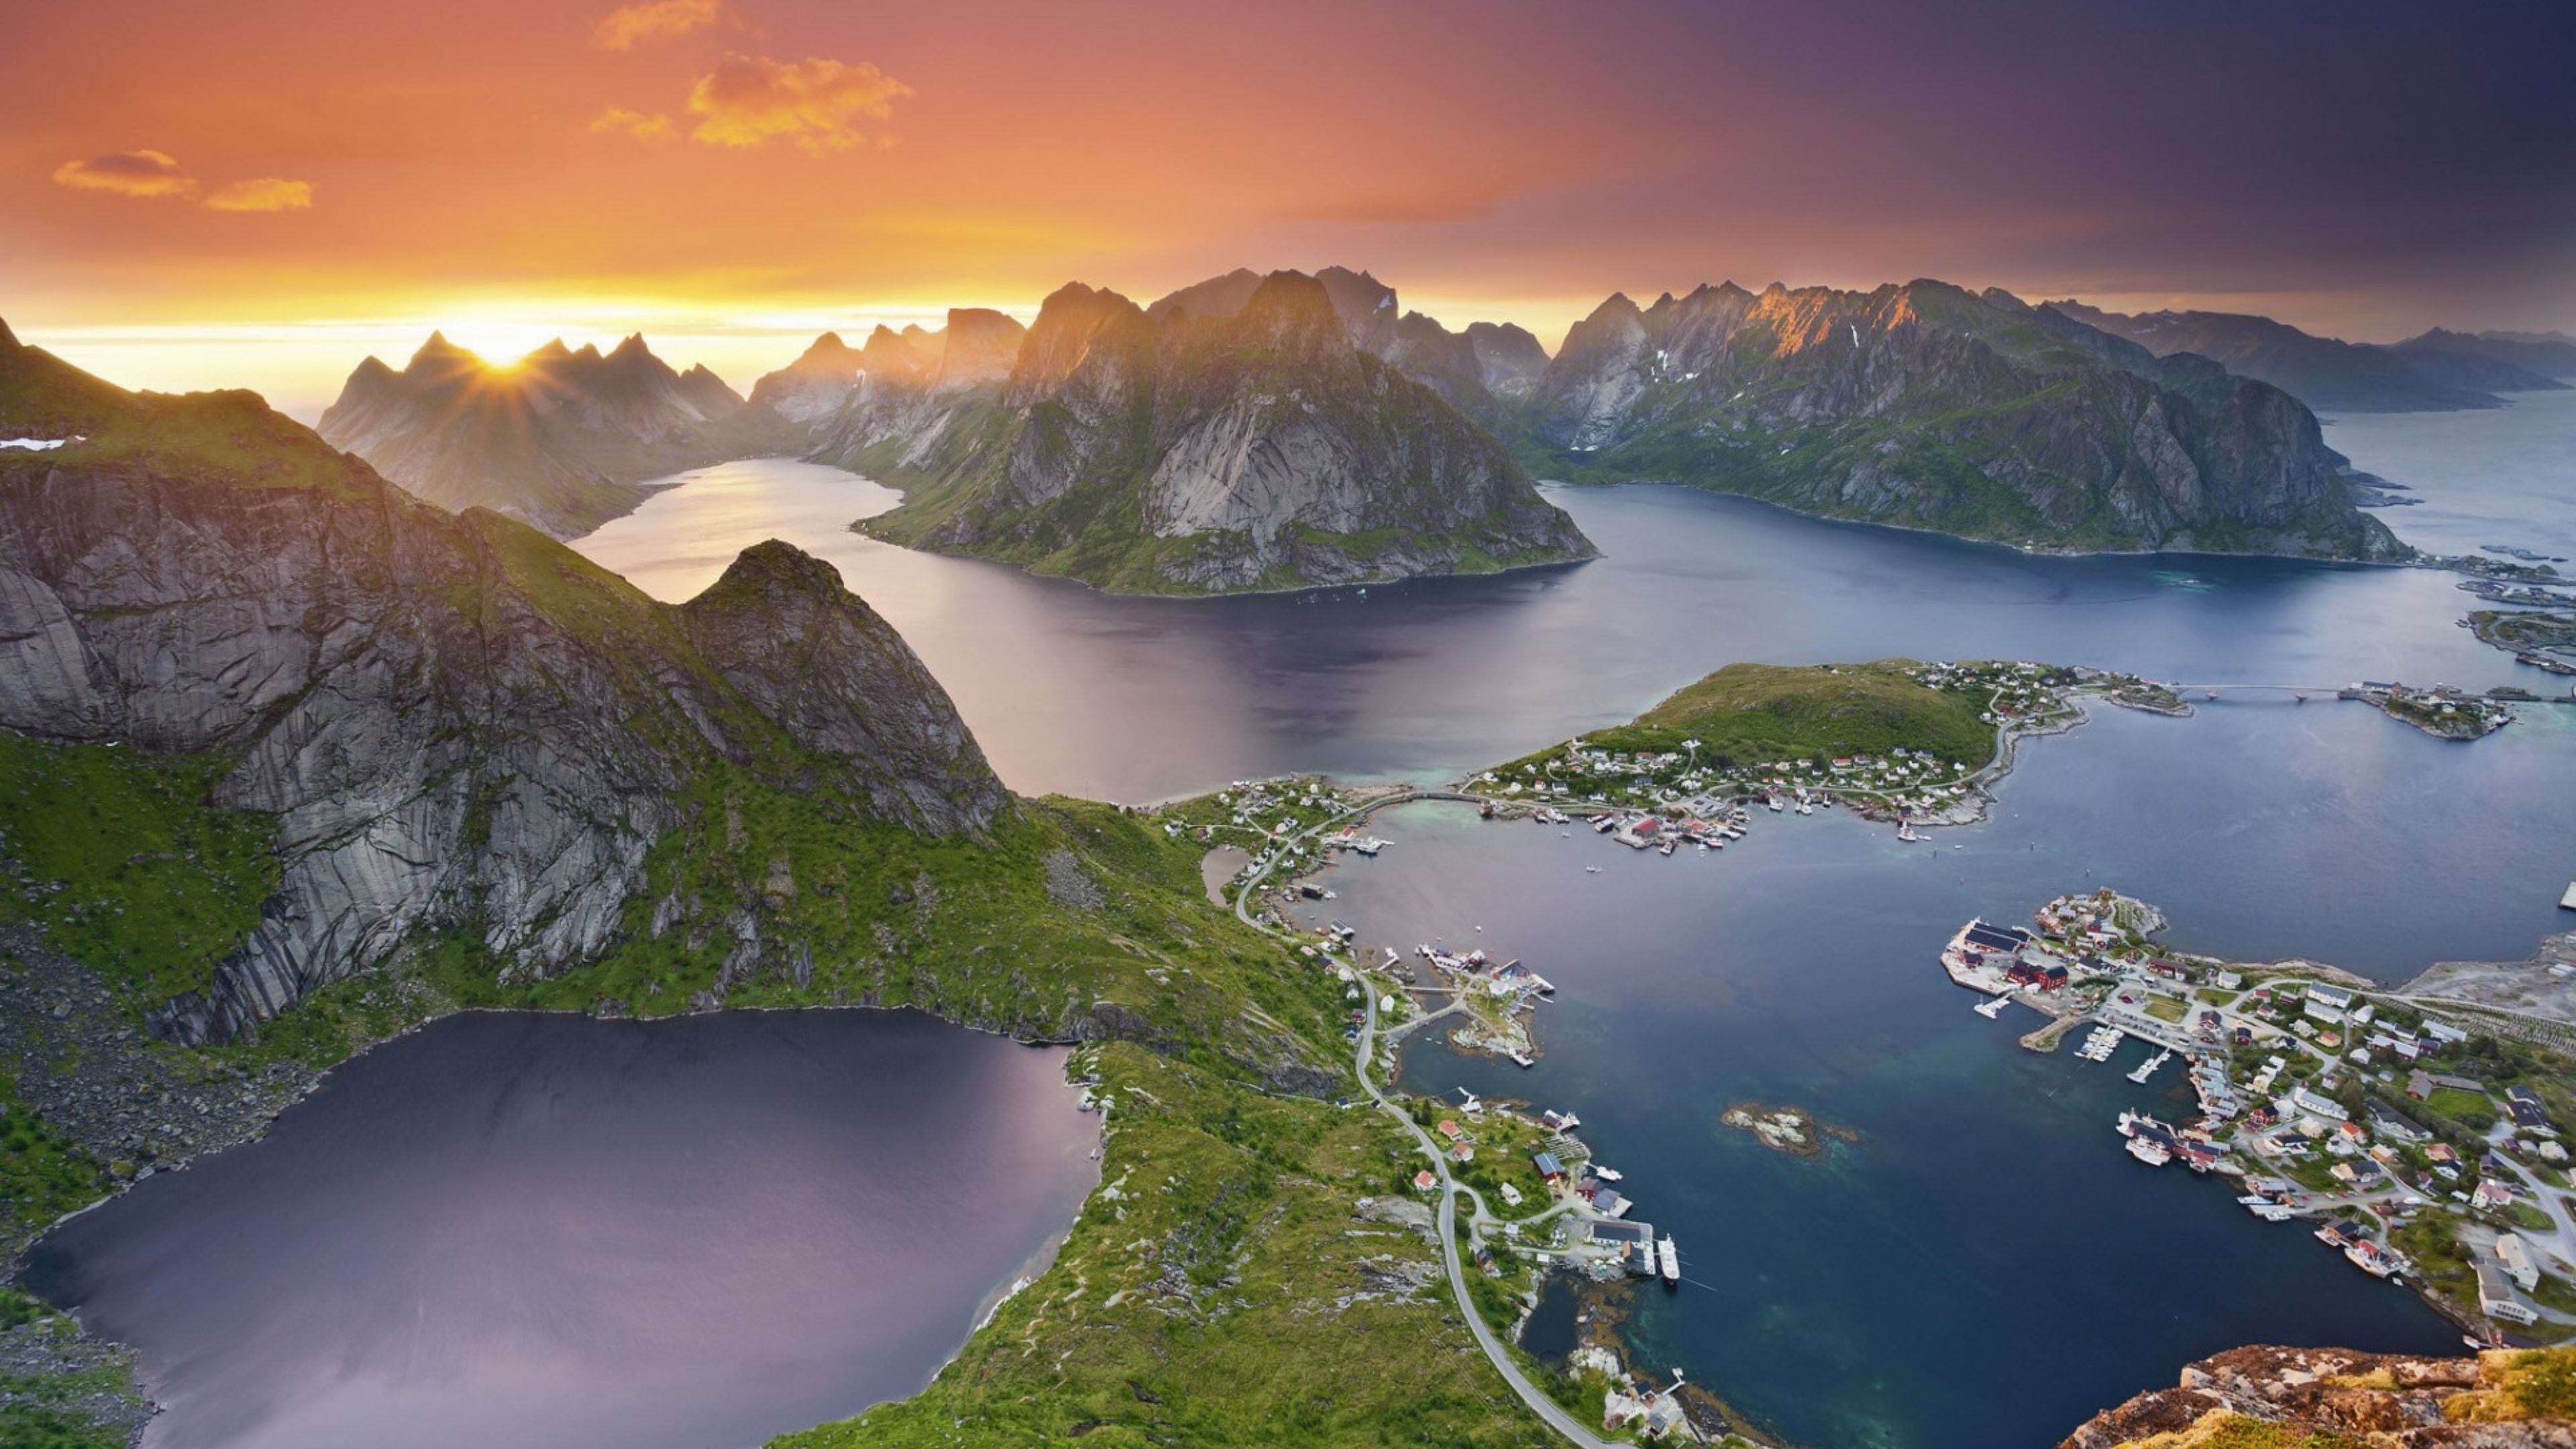
\includegraphics[width=\linewidth]{imgs/Norge1.jpg}
		\caption{Norge 2}
	\end{subfigure}
	\caption{Norge Twice}
	\label{fig:norge}
\end{figure}
Stuffy stuff!
Citation\cite{DUMMY:1} embedded in text.

\subsection{Tables}
\begin{table}[h!]
  \begin{center}
    \caption{Your first table.}
    \label{tab:table1}
    \begin{tabular}{l|c|r} % <-- Alignments: 1st column left, 2nd middle and 3rd right, with vertical lines in between
      \textbf{Value 1} & \textbf{Value 2} & \textbf{Value 3}\\
      $\alpha$ & $\beta$ & $\gamma$ \\
      \hline
      1 & 1110.1 & a\\
      2 & 10.1 & b\\
      3 & 23.113231 & c\\
    \end{tabular}
  \end{center}
\end{table}

\begin{table} [h!]
  \begin{center}
    \caption{Better Rounding}
    \label{tab:table2}
    \begin{tabular}{l|S|r} % <-- Alignments: 1st column left, 2nd middle and 3rd right, with vertical lines in between
      \textbf{Value 1} & \textbf{Value 2} & \textbf{Value 3}\\
      $\alpha$ & $\beta$ & $\gamma$ \\
      \hline
      1 & 1110.1 & a\\
      2 & 10.1 & b\\
      3 & 23.113231 & c\\
    \end{tabular}
  \end{center}
\end{table}

\begin{table} [h!]
  \begin{center}
    \caption{More Rows.}
    \label{tab:table3}
    \begin{tabular}{l|S|r} % <-- Alignments: 1st column left, 2nd middle and 3rd right, with vertical lines in between
      \textbf{Value 1} & \textbf{Value 2} & \textbf{Value 3}\\
      $\alpha$ & $\beta$ & $\gamma$ \\
      \hline
      1 & 1110.1 & a\\
      2 & 10.1 & b\\
      3 & 23.113231 & c\\
      4 & 25.113231 & d\\
    \end{tabular}
  \end{center}
\end{table}

\begin{table} [h!]
  \begin{center}
    \caption{More Columns.}
    \label{tab:table4}
    \begin{tabular}{l|S|r|l} % <-- Alignments: 1st column left, 2nd middle and 3rd right, with vertical lines in between
      \textbf{Value 1} & \textbf{Value 2} & \textbf{Value 3} & \textbf{Value 4}\\
      $\alpha$ & $\beta$ & $\gamma$  & $\delta$ \\
      \hline
		1 & 1110.1 & a & e\\
      2 & 10.1 & b & f\\
      3 & 23.113231 & c & g\\
    \end{tabular}
  \end{center}
\end{table}

% \begin{table} [h!]
%   \begin{center}
%     \caption{Multirow Table.}
%     \label{tab:table1}
%     \begin{tabular}{l|S|r} % <-- Alignments: 1st column left, 2nd middle and 3rd right, with vertical lines in between
%       \textbf{Value 1} & \textbf{Value 2} & \textbf{Value 3}\\
%       $\alpha$ & $\beta$ & $\gamma$ \\
%       \hline
%       \multirow{2}{*}{12} & 1110.1 & a\\
%       & 10.1 & b\\
% 	  \hline
%       3 & 23.113231 & c\\
%       4 & 25.113231 & d\\
%     \end{tabular}
%   \end{center}
% \end{table}

% \begin{table} [h!]
%   \begin{center}
%     \caption{Multicolumn table.}
%     \label{tab:table1}
%     \begin{tabular}{l|S|r}
%       \textbf{Value 1} & \textbf{Value 2} & \textbf{Value 3}\\
%       $\alpha$ & $\beta$ & $\gamma$ \\
%       \hline
%       \multicolumn{2}{c|}{12} & a\\ % <-- Combining two cells with alignment c| and content 12.
%       \hline
%       2 & 10.1 & b\\
%       3 & 23.113231 & c\\
%       4 & 25.113231 & d\\
%     \end{tabular}
%   \end{center}
% \end{table}

% \begin{table} [h!]
%   \begin{center}
%     \caption{Multirow and -column table.}
%     \label{tab:table1}
%     \begin{tabular}{l|S|r}
%       \textbf{Value 1} & \textbf{Value 2} & \textbf{Value 3}\\
%       $\alpha$ & $\beta$ & $\gamma$ \\
%       \hline
%       \multicolumn{2}{c|}{\multirow{2}{*}{1234}} & a\\ % <-- Multicolumn spanning 2 columns, content multirow spanning two rows
%       \multicolumn{2}{c|}{} & b\\ % <-- Multicolumn spanning 2 columns with empty content as placeholder
%       \hline
%       3 & 23.113231 & c\\
%       4 & 25.113231 & d\\
%     \end{tabular}
%   \end{center}
% \end{table}

% Booktab Example -- Prettier
% \begin{table} [!h]
%   \begin{center}
%     \caption{Table using booktabs.}
%     \label{tab:table1}
%     \begin{tabular}{l|S|r}
%       \toprule % <-- Toprule here
%       \textbf{Value 1} & \textbf{Value 2} & \textbf{Value 3}\\
%       $\alpha$ & $\beta$ & $\gamma$ \\
%       \midrule % <-- Midrule here
%       1 & 1110.1 & a\\
%       2 & 10.1 & b\\
%       3 & 23.113231 & c\\
%       \bottomrule % <-- Bottomrule here
%     \end{tabular}
%   \end{center}
% \end{table}

% \newpage
% \begin{sidewaystable}[h!] % <--
%   \thispagestyle{empty}
%   \begin{center}
%   \caption{Landscape table.}
%   \label{tab:table4}
%   \begin{tabular}{l|S|r}
%       \toprule
%       \textbf{Value 1} & \textbf{Value 2} & \textbf{Value 3}\\
%       $\alpha$ & $\beta$ & $\gamma$ \\
%     \midrule
%     1 & 1110.1 & a\\
%     2 & 10.1 & b\\
%     3 & 23.113231 & c\\
%     \bottomrule
%   \end{tabular}
%   \end{center}
% \end{sidewaystable}


\newpage

\bibliography{tst}
\bibliographystyle{ieeetr}
\end{document}

